% Prof. Dr. Ausberto S. Castro Vera
% UENF - CCT - LCMAT - Curso de Ci\^{e}ncia da Computa\c{c}\~{a}o
% Campos, RJ,  2022
% Disciplina: Paradigmas de Linguagens de Programa\c{c}\~{a}o
% Aluno: Ricardo Willian Pontes da Silva



\chapter{ Aplica\c{c}\~{o}es da Linguagem Python}

No capítulo a seguir serão apresentadas cinco aplica\c{c}\~{o}es completas na linguagem Python, contento:
\begin{itemize}
  \item Uma breve descri\c{c}\~{a}o da aplica\c{c}\~{a}o
  \item O c\'{o}digo completo da aplica\c{c}\~{a}o,
  \item Imagens do c\'{o}digo fonte no compilador-interpretador,
  \item Imagens dos resultados ap\'{o}s a compila\c{c}\~{a}o-interpreta\c{c}\~{a}o do c\'{o}digo fonte
  \item Links e referencias bibliogr\'{a}ficas de onde foi obtido a aplica\c{c}\~{a}o
\end{itemize}




    \section{Opera\c{c}\~{o}es b\'{a}sicas}


    \section{Programas gr\'{a}ficos}
A linguagem Python é altamente permissiva a manipulação de dados, e com isso existem ferramentas que se utilizam desse estudo de informações, como a criação de gráficos. Para isso é necessário a utilização da biblioteca Matplotlib que é basicamente uma ferramenta para criação de gráficos e visualização dos mesmos.

\begin{lstlisting}
import sys
import matplotlib
matplotlib.use('Agg')

import matplotlib.pyplot as plt
import numpy as np

x = np.array(["prova1","prova2","prova3","prova4"])
y = np.array([3, 8, 1, 10])

plt.plot(x, y)
plt.show()
plt.savefig(sys.stdout.buffer)
sys.stdout.flush()

	
\end{lstlisting}
  
  \begin{figure}[H]
  	\begin{center}
  		\caption{Gráfico gerado pela biblioteca matplotlib} \label{ling1}
  		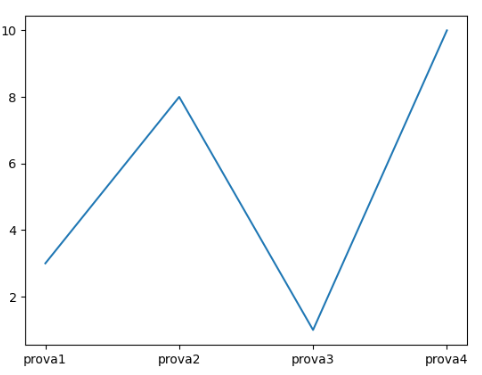
\includegraphics[width=9cm]{grafico py.PNG} \\
  		{\tiny \sf Fonte:{ Autor}}
  	\end{center}
  \end{figure}
  
    \section{Programas com Objetos}


    \section{O algoritmo Quicksort - Implementa\c{c}\~{a}o}

O Quicksort é um famoso algoritmo de ordenação que tem como filosofia dividir para conquistar, ou seja, ele utilizasse de ordenação por troca recursiva onde a entrada do algoritmo é difundida diversas vezes com o objetivo de transformar em problemas menores.

\begin{lstlisting}
def quickSort(alist):
quickSortHelper(alist,0,len(alist)-1)

def quickSortHelper(alist,first,last):
if first<last:

splitpoint = partition(alist,first,last)

quickSortHelper(alist,first,splitpoint-1)
quickSortHelper(alist,splitpoint+1,last)


def partition(alist,first,last):
pivotvalue = alist[first]

leftmark = first+1
rightmark = last

done = False
while not done:

while leftmark <= rightmark and alist[leftmark] <= pivotvalue:
leftmark = leftmark + 1

while alist[rightmark] >= pivotvalue and rightmark >= leftmark:
rightmark = rightmark -1

if rightmark < leftmark:
done = True
else:
temp = alist[leftmark]
alist[leftmark] = alist[rightmark]
alist[rightmark] = temp

temp = alist[first]
alist[first] = alist[rightmark]
alist[rightmark] = temp


return rightmark

alist = [100,2,93,1,31,77,44,5,20]
quickSort(alist)
print(alist)
	
\end{lstlisting}

\begin{figure}[H]
	\begin{center}
		\caption{Execução do algoritmo Quicksort na linguagem Python} \label{ling1}
		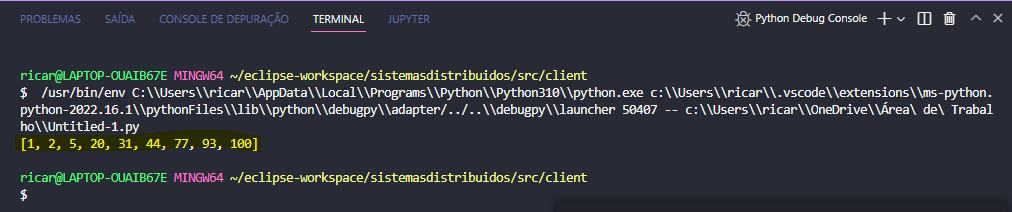
\includegraphics[width=9cm]{quicksort.PNG} \\
		{\tiny \sf Fonte:{ Autor}}
	\end{center}
\end{figure}

    \section{Aplica\c{c}\~{o}es com Banco de Dados}
Um banco de dados é mm conjunto de arquivos inter-relacionados, ou seja, são coleções organizadas de dados que se relacionam de forma significativa e proporcionam maior eficiência durante a pesquisa ou estudo científico. A linguagem Python possui integração com as principais linguagens de banco de dados como a Sql, que será utilizada para elucidar os exemplos. Para trabalhar com banco de dados na linguagem Python é necessário baixar o conector mysql. O exemplo abaixo tem como objetivo ilustrar a criação de um banco de dados simples e mostrar que o mesmo foi criado satisfatoriamente.

\begin{lstlisting}
import mysql.connector
	
mydb = mysql.connector.connect(
host="localhost",
user="Ricardo Pontes",
password="PLP2022"
)

mycursor = mydb.cursor()
mycursor.execute("SHOW DATABASES")
	
for x in mycursor:
  print(x)
	
\end{lstlisting}

Abaixo será apresentado mais um trecho de código com o objetivo de elucidar a criação de uma tabela simples utilizando a linguagem Python e Mysql.

\begin{lstlisting}

import mysql.connector

mydb = mysql.connector.connect(
host="localhost",
user="Ricardo Pontes",
password="PLP2022",
database="mydatabase"
)

mycursor = mydb.cursor()

sql = "INSERT INTO customers (nome, endereco) VALUES (%s, %s)"
val = ("Ricardo Willian Pontes da Silva", "Alberto Lamego")

mycursor.execute(sql, val)

mydb.commit()

print(mycursor.rowcount, "record inserted.")
	
\end{lstlisting}

 \begin{figure}[H]
	\begin{center}
		\caption{criação de uma tabela utilizando a linguagem Python e Mysql} \label{ling1}
		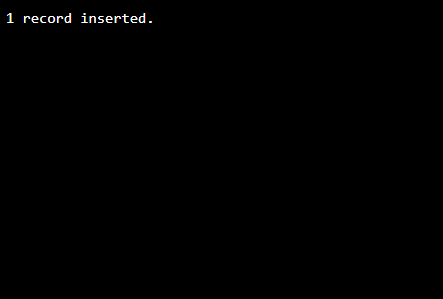
\includegraphics[width=9cm]{database.PNG} \\
		{\tiny \sf Fonte:{ Autor}}
	\end{center}
\end{figure}
